\documentclass[
  shownotes,
  xcolor={svgnames},
  hyperref={colorlinks,citecolor=DarkBlue,linkcolor=DarkRed,urlcolor=DarkBlue}
  , aspectratio=169]{beamer}
\usepackage{animate}
\usepackage{amsmath}
\usepackage{amsfonts}
\usepackage{amssymb}
\usepackage{pifont}
\usepackage{mathpazo}
%\usepackage{xcolor}
\usepackage{multimedia}
\usepackage{fancybox}
\usepackage[para]{threeparttable}
\usepackage{multirow}
\setcounter{MaxMatrixCols}{30}
\usepackage{subcaption}
\usepackage{graphicx}
\usepackage{lscape}
\usepackage[compatibility=false,font=small]{caption}
\usepackage{booktabs}
\usepackage{ragged2e}
\usepackage{chronosys}
\usepackage{appendixnumberbeamer}
\usepackage{animate}
\setbeamertemplate{caption}[numbered]
\usepackage{color}
%\usepackage{times}
\usepackage{tikz}
\usepackage{comment} %to comment
%% BibTeX settings
\usepackage{natbib}
\bibliographystyle{apalike}
\bibpunct{(}{)}{,}{a}{,}{,}
\setbeamertemplate{bibliography item}{[\theenumiv]}

% Defines columns for bespoke tables
\usepackage{array}
\newcolumntype{L}[1]{>{\raggedright\let\newline\\\arraybackslash\hspace{0pt}}m{#1}}
\newcolumntype{C}[1]{>{\centering\let\newline\\\arraybackslash\hspace{0pt}}m{#1}}
\newcolumntype{R}[1]{>{\raggedleft\let\newline\\\arraybackslash\hspace{0pt}}m{#1}}


\usepackage{xfrac}


\usepackage{multicol}
\setlength{\columnsep}{0.5cm}

% Theme and colors
\usetheme{Boadilla}

% I use steel blue and a custom color palette. This defines it.
\definecolor{andesred}{HTML}{af2433}

% Other options
\providecommand{\U}[1]{\protect\rule{.1in}{.1in}}
\usefonttheme{serif}
\setbeamertemplate{itemize items}[default]
\setbeamertemplate{enumerate items}[square]
\setbeamertemplate{section in toc}[circle]

\makeatletter

\definecolor{mybackground}{HTML}{82CAFA}
\definecolor{myforeground}{HTML}{0000A0}

\setbeamercolor{normal text}{fg=black,bg=white}
\setbeamercolor{alerted text}{fg=red}
\setbeamercolor{example text}{fg=black}

\setbeamercolor{background canvas}{fg=myforeground, bg=white}
\setbeamercolor{background}{fg=myforeground, bg=mybackground}

\setbeamercolor{palette primary}{fg=black, bg=gray!30!white}
\setbeamercolor{palette secondary}{fg=black, bg=gray!20!white}
\setbeamercolor{palette tertiary}{fg=white, bg=andesred}

\setbeamercolor{frametitle}{fg=andesred}
\setbeamercolor{title}{fg=andesred}
\setbeamercolor{block title}{fg=andesred}
\setbeamercolor{itemize item}{fg=andesred}
\setbeamercolor{itemize subitem}{fg=andesred}
\setbeamercolor{itemize subsubitem}{fg=andesred}
\setbeamercolor{enumerate item}{fg=andesred}
\setbeamercolor{item projected}{bg=gray!30!white,fg=andesred}
\setbeamercolor{enumerate subitem}{fg=andesred}
\setbeamercolor{section number projected}{bg=gray!30!white,fg=andesred}
\setbeamercolor{section in toc}{fg=andesred}
\setbeamercolor{caption name}{fg=andesred}
\setbeamercolor{button}{bg=gray!30!white,fg=andesred}

\makeatother


%%%%%%%%%%%%%%% BEGINS DOCUMENT %%%%%%%%%%%%%%%%%%

\begin{document}

\title{Lecture 1: Introducción}
\subtitle{Big Data and Machine Learning for Applied Economics \\ Econ 4676}
\date{\today}

\author[Sarmiento-Barbieri]{Ignacio Sarmiento-Barbieri}
\institute[Uniandes]{Universidad de los Andes}


\begin{frame}[noframenumbering]
\maketitle
\end{frame}

%%%%%%%%%%%%%%%%%%%%%%%%%%%%%%%%%%%
%       Motivation              %
% What is the question?
% Why do we care?
% What is new?
% What do you find?
%%%%%%%%%%%%%%%%%%%%%%%%%%%%%%%%%%%




\begin{frame}
\frametitle{Agenda}

\tableofcontents


\end{frame}


%----------------------------------------------------------------------%
\section{Motivación}
\subsection{Ejemplos para Motivarnos}

\begin{frame}
\frametitle{Motivación}
\framesubtitle{La primera victoria y derrota del Big Data}

\begin{itemize}
  \item Contexto ?`similar? al de hoy: Epidemia de la gripe A en 2009
  \medskip
  \item En EEUU la forma de monitorear es a través de reportes de la CDC 
  \medskip
  \item La CDC agrega a nivel de ciudad, condado, estado, región y a nivel nacional
  \medskip
  \item Todo esto llevaba aproximadamente 10 días $\rightarrow$ demasiado tiempo para una epidemia
\end{itemize}
\end{frame}

%----------------------------------------------------------------------%

\begin{frame}
\frametitle{Motivación}
\framesubtitle{Google se ha unido a la conversación}

\begin{itemize}
  \item Google propuso un mecanismo ingenioso: {\bf Google Flu Trends}
  \bigskip
  \item Punto de partida: 
  \begin{itemize}
    \item Proporcion de visitas semanales por Gripe A en hospitales 
    \item 9 regiones $\times$ 5 años (2003-2007) = $2,340$ datos
    \item Estos son los datos que tomaban 10 dias en elaborarse (comparemos con la Colombia de 2009)
  \end{itemize}
  \bigskip
  \item Google cruzó estos datos con las busquedas sobre la gripe A
  \bigskip
  \item Con estos datos, construyeron un modelo para predecir intensidad de gripe A  
\end{itemize}  

\end{frame}

%----------------------------------------------------------------------%

\begin{frame}
\frametitle{Motivación}
\framesubtitle{Google se ha unido a la conversación}

\begin{itemize}
  \item Un solo modelo?
  \bigskip
  \item Los investigadores de Google estimaron {\bf 450 millones} de models
  \bigskip
  \item Eligieron el que mejor predice sobe la intensidad de busqueda
  \bigskip
  \item Les permite tener informacion diaria, semanal o mensual para cualquier punto de EEUU y el mundo
  \bigskip
  \item A Google le toma 1 día lo que a la CDC 10!
\end{itemize}  
\end{frame}



%----------------------------------------------------------------------%

\begin{frame}
\frametitle{Motivación}
\framesubtitle{Google se ha unido a la conversación}
\begin{figure}[H] \centering
            \captionsetup{justification=centering}  
            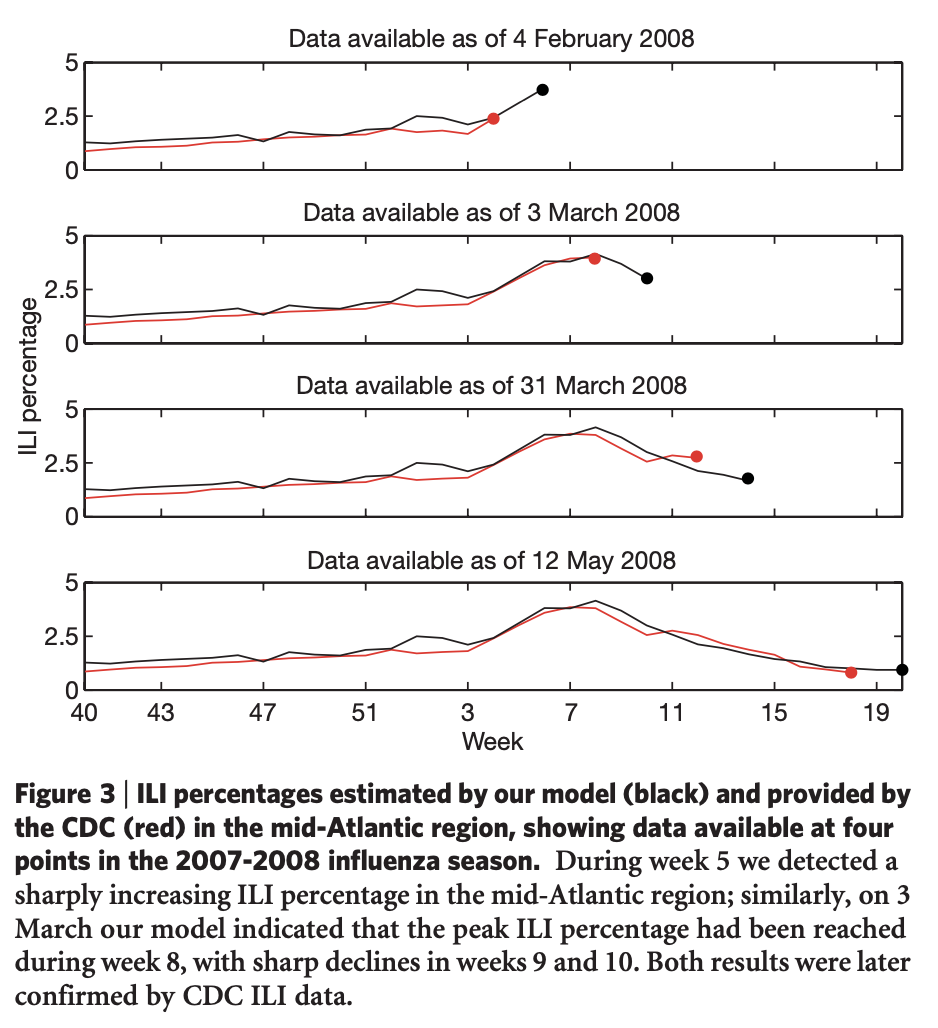
\includegraphics[scale=0.45]{figures/flu_trends}
    \end{figure}
\end{frame}


%----------------------------------------------------------------------%

\begin{frame}
\frametitle{Motivación}
\framesubtitle{El rey ha muerto, larga vida al rey}
  \begin{itemize}
    \item Qué tienen en común Google Flu y Elvis?
    \bigskip
    \begin{itemize}
      \item Abanderados de la revolución
      \medskip
      \item Definió y redefinió las reglas sistemáticas para hallar la solución a un problema
      \medskip
      \item Éxito rotundo $\rightarrow$ Publicacion en Nature! \url{https://www.nature.com/articles/nature07634}
      \medskip
      \item Pero como a Elvis el éxito fue efímero
      \medskip
      \item La predicciones comenzaron a sobre-estimar considerablemente la incidencia de la gripe A
      \medskip
      \item Google Flu esta ahora archivado (disponible al publico)
      \medskip
      \item Continúa recolectando datos pero solo algunas instituciones científicas tienen accesso 
    \end{itemize}  
  \end{itemize}  
\end{frame}
%----------------------------------------------------------------------%

\begin{frame}
\frametitle{Motivación}

\begin{itemize}
      \item Otro ejemplo, los algoritmos de reconocimiento de cara: 
      \medskip
      \begin{itemize}
        \item no son reglas fijas basadas en que los humanos entendemos por rostros y a partir de ello buscar combinaciones de pixeles.
        \item son algoritmos que usan datos de fotos etiquetadas con un rostro y estiman una funcion $f(x)$ que predice si es un rostro o no a partir de pixeles x.
      \end{itemize}
      \medskip
      \item El aprendizaje de maquinas se hizo una realidad cuando los investigadores dejaron de afrontarlo de manera teórica y lo hicieron empíricamente.
      \medskip
      \item  Las similitudes con la econometría plantea interrogantes:
      \begin{itemize}
      \item  ¿Estos algoritmos están simplemente aplicando técnicas estándar a nuevos y grandes conjuntos de datos? 
      \item  Si hay herramientas empíricas fundamentalmente nuevas, ¿cómo encajan con lo que conocemos? 
      \item  Como economistas empíricos, ¿cómo podemos utilizarlas?
       \end{itemize}
\end{itemize}

\end{frame}

%%----------------------------------------------------------------------%

\subsection{¿Qué entendemos por Big Data y ML?}
\begin{frame}
\frametitle{¿Qué entendemos por Big Data y ML?}

\begin{figure}[H] \centering
  \captionsetup{justification=centering}  
    
\includegraphics[scale=0.5]{figures/data_everywhere}
\end{figure}



\end{frame}

%----------------------------------------------------------------------%
\begin{frame}
\frametitle{¿Qué entendemos por Big Data y ML?}

\begin{itemize}
      \item ¿Que es Big Data? 
      \begin{itemize}
      \item Big n, es solo parte de la historia
      \item Big también es big k, muchos covariates, a veces $n<<k$
      \item Vamos a entender Big también como datos que no surgen de fuentes tradicionales (cuentas nac., GEIH, etc)
      \begin{itemize}
        \item Datos de la Web
        \item GPS
        \item Texto
        \item Imágenes
      \end{itemize}
      \end{itemize}
      \medskip
      \item Machine Learning
        \begin{itemize}
          \item Cambio de paradigma de estimación a predicción

        \end{itemize} 
      
\end{itemize}

\end{frame}

%----------------------------------------------------------------------%

\section{Presentación: un poco sobre nosotros}
\begin{frame}
\frametitle{Presentación: Sobre mi}

  \begin{itemize}
      \item  Ignacio Sarmiento Barbieri
      \medskip
      \item \url{https://ignaciomsarmiento.github.io/}
      \medskip
      \item \href{mailto:i.sarmiento@uniandes.edu.co}{i.sarmiento@uniandes.edu.co}
      \medskip
      \item Intereses: Economia Pública y Urbana. Economia del Crime. Econometria Aplicada, Big Data y Machine Learning.
      \medskip
      \item Originario de Salta, Argentina
  \end{itemize}

\end{frame}

%----------------------------------------------------------------------%

\begin{frame}
\frametitle{Presentación: Sobre el profesor asistente del curso}

  \begin{itemize}
      \item  Rafael Cano Polania
      \medskip
      \item \href{mailto:r.cano@uniandes.edu.co}{r.cano@uniandes.edu.co}
      \medskip
      \item Intereses: Big Data y Machine learning, Web scraping, text analysis, Deep Learning, NlP y algorithmic programing
      \medskip
      \item Clases Viernes 3:00 pm

  \end{itemize}

\end{frame}


%----------------------------------------------------------------------%
\section{Housekeeping}
\begin{frame}
\frametitle{Clases}


    \begin{itemize}
      \item Horario de Clases: Las clases serán completamente virtuales los martes y jueves a las 2pm
      \bigskip
      \item Zoom link: \url{https://uniandes-edu-co.zoom.us/j/81357439760}
      \bigskip
      \item Github classrooms \url{https://github.com/ECON-4676-UNIANDES-Fall-2021}
      \begin{itemize}
        \item Syllabus: \url{https://github.com/ECON-4676-UNIANDES-Fall-2021/Syllabus}
        \item Clases
        \item Talleres
        \item Tutoriales (eTAs)
        \end{itemize}
      \bigskip
      \item Comunicacion via \href{https://slack.com/}{Slack}. Si no recibieron el link de la invitación por favor enviarme correo
    \end{itemize}


\end{frame}

%----------------------------------------------------------------------%

\begin{frame}
\frametitle{Lenguajes}


\begin{minipage}[t]{0.58\linewidth}
        \begin{itemize}
            \item Matemáticas
            \bigskip
            \item Inglés
            \bigskip
            \item Uno de los objetivos implicitos es que mejoren sus habilidades para escribir código y usar herramientas de la industria
            \begin{itemize}
              \item Elijan el que quieran: 
              \begin{itemize}
                \item \texttt{R}, \texttt{Python}, o cualquier otro
                \item no hay restricción
                \item yo me basare en \texttt{R}, Rafael en \texttt{Python}
                \end{itemize}
              \item Github
              \item Azure y AWS
            \end{itemize}
            \item Aprender haciendo y mucha prueba y error! 
            
        \end{itemize}
    \end{minipage}
    \hfill
    \begin{minipage}[t]{0.38\linewidth}%
        \begin{figure}[H] \centering
            \captionsetup{justification=centering}  
            
\includegraphics[scale=0.2]{figures/ml_trick}
    \end{figure}
    \end{minipage}

\end{frame}

%----------------------------------------------------------------------%

\begin{frame}
\frametitle{Bibliografía}


\begin{enumerate}
  \item Statistical Learning (FREE!!! speech and beer) \url{https://www.gnu.org/philosophy/free-sw.en.html}
  \begin{itemize}
    \small
    \item James, G., Witten, D., Hastie, T., \& Tibshirani, R. (2013). An introduction to statistical learning (ISLR)
    \item Hastie, T., Tibshirani, R., \& Friedman, J. (2009). The elements of statistical learning: data mining, inference, and prediction
    \item Efron, B., \& Hastie, T. (2016). Computer age statistical inference.
  \end{itemize}
  \bigskip
  \item Libros avanzados de econometría
  \begin{itemize}
    \small
    \item Davidson, R., \& MacKinnon, J. G. (2004). Econometric theory and methods 
    \item Wooldridge, J. M. (2010). Econometric analysis of cross section and panel data. 
    \item Hayashi, F. (2000). Econometrics
  \end{itemize}
\bigskip
  \end{enumerate}



%  \begin{itemize}
%    \item La idea es movernos hacia adelante y al costado de la econometria de grado
%    \item Armar un puente entre los Economistas y los Machine Learners, Computer Scientists
%    \item Pensar el curso como un ISLR/Elements pero para economistas
%\end{itemize}


\end{frame}
%----------------------------------------------------------------------%

\begin{frame}
\frametitle{Criterios de evaluación}

\begin{table}[H]
\centering
\caption{Puntajes}
\scriptsize
\begin{tabular}{lccc}
\hline
 \hline
\multicolumn{2}{l}{}                       & Puntaje Individual & Puntaje Total \\
\multicolumn{2}{l}{Participación}          &                    & 10\%          \\
\multicolumn{2}{l}{Talleres}               & 10\%               & 60\%          \\
\multicolumn{2}{l}{Trabajo Final}        &                    & 30\%          \\
              & Primer Entrega             & 5\%                &               \\
              & Presentaciones             & 10\%               &               \\
               & Entrega Final            & 15\%               &               \\
\multicolumn{2}{l}{Total}                  &                    & 100\%        \\
\hline
 \hline
\end{tabular}
\end{table}


\end{frame}


%----------------------------------------------------------------------%

\begin{frame}
\frametitle{Criterios de evaluación}

\begin{itemize}
\item {\bf Participación (10\%)} $\rightarrow$ ``tiebreaker'' de la nota final. 
\medskip
  \begin{itemize}
    \item Asistencia a clases: aleatoriamente voy a asignar al menos 4 personas que tengan la camara prendida, voy a mandar mensaje por Slack
    \medskip
    \item Slack: compartir articulos, tutoriales, material relevante para el curso en el canal \#cosas interesantes
    \medskip
    \item Github: Spell check al instructor, sobre todo acentos =), y corregir falacias/errores conceptuales
    \medskip
    \item Presentacion de los talleres

  \end{itemize}
\end{itemize}

\end{frame}
%----------------------------------------------------------------------%
\begin{frame}
\frametitle{Criterios de evaluación}
\begin{itemize}
  \item {\bf Talleres (60\%)}
  \bigskip
\begin{itemize}
  \item Pueden ser en grupos de no mas de 3 personas. 
  \medskip
  \item Enviar slack al profe con los miembros del grupo
  \medskip
  \item Bonus en participación de la historia del repositorio (evaluar la contribución de cada estudiante).
  \medskip
  \item Voy a elegir aleatoriamente a alguien que presente. Voy a informarles ese dia.
  \end{itemize}
\bigskip

   \item Primer taller $\rightarrow$ fecha de entrega 24 de Agosto 1pm
   
\end{itemize}

\end{frame}
%----------------------------------------------------------------------%
\begin{frame}
\frametitle{Criterios de evaluación}
\begin{itemize}

  \item {\bf Trabajo Final  (30\%)}
  \begin{itemize}
  \item Pueden ser en grupos de no mas de 3 personas. El mismo o no de los talleres.
  \item Ver los \href{https://github.com/ECON-4676-UNIANDES-Fall-2021/Problem_Sets/tree/master/Final_Project}{guidelines}
  \end{itemize}
  \end{itemize}
     \medskip
  \begin{enumerate}
      
      \item Primera entrega escrita 
      \begin{itemize}
        \item 2 paginas max!
        \item fecha de entrega: 22 de Octubre 6pm
      \end{itemize}
  
     \medskip
  \item  Presentaciones
      \begin{itemize}
        \item 15 min (max)
        \item fecha de entrega: ultima semana de clases
      \end{itemize}
      \medskip
    \item  Entrega final que consolida todo el trabajo.
      \begin{itemize}
        \item 5 pag. max!
        \item fecha de entrega:  10 de diciembre 6pm
      \end{itemize}
\end{enumerate}






\end{frame}
%----------------------------------------------------------------------%
\begin{frame}
\frametitle{Cláusula de ajustes razonables}

\begin{itemize}
  \scriptsize
\item  Si lo considera pertinente, siéntase en libertad de informar al profesor lo antes posible si usted tiene alguna condición, visible o invisible, por la cual requiera algún ajuste para estar en igualdad de condiciones con los y las demás estudiantes. Debido a las actuales circunstancias, barreras de conectividad o acceso a los recursos tecnológicos indispensables para la clase son parte de las condiciones que pueden requerir ajustes. Por la misma razón, no necesitará presentar documentación para solicitar esos ajustes.

\item  También lo invitamos a buscar asesoría y apoyo en la Dirección de su programa, en la Decanatura de Estudiantes (http://centrodeconsejeria.uniandes.edu.co, Bloque Ñf, ext. 2207, 2230 y 4967, horario de atención L-V 8:00 a.m. a 5:00 p.m.) o en el Programa de Acción por la Igualdad y la Inclusión Social (PAIIS) de la Facultad de Derecho (paiis@uniandes.edu.co). Si su solicitud se basa en dificultades de acceso a conectividad o tecnología, es particularmente importante que haga este contacto adicional para que pueda acceder a los recursos de apoyo que brinda la Universidad.

\item  Se entiende por ajustes razonables todas "las modificaciones y adaptaciones necesarias y adecuadas que no impongan una carga desproporcionada o indebida, cuando se requieran en un caso particular, para garantizar a las personas con discapacidad el goce o ejercicio, en igualdad de condiciones con las demás, de todos los derechos humanos y libertades fundamentales" Convención sobre los Derechos de las personas con discapacidad, art.2.
\item Si quiere más información sobre ajustes razonables, puede visitar \href{esta página de la DECA}{https://agora.uniandes.edu.co/que-son-los-ajustes-razonables/}. Y sobre la política de momentos difíciles, \href{esta otra}{https://agora.uniandes.edu.co/sabes-que-es-la-politica-de-momentos-dificiles/}.

\end{itemize}
\end{frame}
%----------------------------------------------------------------------%
\begin{frame}
\frametitle{Cláusula de respeto por la diversidad}

\begin{itemize}
  \footnotesize
\item  Todos debemos respetar los derechos de quienes hacemos parte de esta comunidad académica. En esta comunidad consideramos inaceptable cualquier situación de acoso, acoso sexual, discriminación, matoneo, y/o amenaza.
La persona que se sienta en alguna de estas situaciones puede denunciar su ocurrencia y buscar orientación y apoyo ante alguna de las siguientes instancias:
\begin{itemize}
  \scriptsize
\item El equipo pedagógico de este curso, la Coordinación o la Dirección del programa de Economía. 
\item La Decanatura de Estudiantes (DECA, Ed. Ñf-Casita amarilla).
\item La Ombudsperson (\href{mailto:ombudsperson@uniandes.edu.co}{ombudsperson@uniandes.edu.co}, Edificio RGA–Pedro Navas, Of. 201, ext. 5300 y 3933).
\item El Comité MAAD (\href{mailto:lineamaad@uniandes.edu.co}{lineamaad@uniandes.edu.co}, \url{https://uniandes.edu.co/MAAD} o a la ext. 2707 o 2230). Si quieren mayor información, guía o necesitan activar el protocolo MAAD pueden acudir a Nancy García (\href{mailto:n.garcia@uniandes.edu.co}{n.garcia@uniandes.edu.co}) en la Facultad. Para mayor información sobre el protocolo MAAD, puede visitar esta página: \url{https://decanaturadeestudiantes.uniandes.edu.co/index.php/es/sobre-la-decanatura/827}
\item Grupos de apoyo estudiantiles que pueden ofrecerle apoyo y acompañamiento: No Es Normal (\href{mailto:derechoygenero@uniandes.edu.co}{derechoygenero@uniandes.edu.co} o \url{https://www.facebook.com/noesnormaluniandes/?fref=ts}); Pares de Acompañamiento Contra el Acoso-PACA (\href{mailto:paca@uniandes.edu.co}{paca@uniandes.edu.co} o \url{https://www.facebook.com/PACA- 1475960596003814/?fref=ts}).
\item Para mayor información sobre el protocolo MAAD, puede visitar esta página: \url{https://agora.uniandes.edu.co/wp-content/uploads/2020/09/ruta-maad.pdf}


\end{itemize}
\end{itemize}
\end{frame}
%----------------------------------------------------------------------%
\begin{frame}
\frametitle{Política de momentos difíciles}

\begin{itemize}
\item Todas las personas pueden pasar por un momento difícil que de alguna manera pueda afectar nuestra vida en la Universidad. Pueden ser problemas en casa, con la pareja, incluso estrés por esta u otra materia.
\medskip
\item Si usted siente que está pasando por un momento complicado, sin importar el motivo, siéntase con la tranquilidad de hablar con la profesora para pedir tiempo o apoyo. Ningún trabajo o entrega puede sobrepasar su salud mental y física.
\medskip
 \item {\bf Su bienestar es lo más importante.}
\end{itemize}
\end{frame}

%----------------------------------------------------------------------%

\section{Recap}
\begin{frame}
\frametitle{Recap}

\begin{itemize} 
  \item 3 Plataformas
    \begin{itemize} 
      \item Curso: Github \url{https://github.com/ECON-4676-UNIANDES-Fall-2021}
      \item Comunicación: Slack
      \item Play: AWS y Azure
    \end{itemize}
    \medskip
    \item Inglés, Estadística, Econometria y mucho coding
    \medskip
    \item Participación, prueba y error serán las banderas del curso, armarse de paciencia!
    \medskip
    \item No duden en comunicarse conmigo por cualquier tema
    \begin{itemize} 
      \item Ajustes razonables, incluyendo problemas de conectividad
      \item Consultas del curso o de cualquier otra cosa
      \item Momentos difíciles 
    \end{itemize}
    \bigskip
    \item {\bf Recordar: Tu bienestar es lo más importante!!!}
\end{itemize}
\end{frame}



%----------------------------------------------------------------------%

\section{Next}

\begin{frame}
\frametitle{Next}
  
  \begin{itemize} 
  \item Cambio de Paradigma: paradigma predictivo
  \bigskip
  \item Nota: En la clases voy a usar ejemplos en \texttt{R} con \texttt{RStudio}
  \medskip
    \begin{itemize} 
      \item Usted puede usar el que desee, altamente recomendados son \texttt{R} y \texttt{Python} 
      \medskip
      \item Rafael va a usar \texttt{Python} 
      \medskip
      \item Tutorial de \texttt{R}  y \texttt{Python}  disponible en los e-TAs
      \medskip
      \item Sera muy bienvenido y debidamente atribuido si quiere contribuir con los tutorials ya sea en  \texttt{Python}  o \texttt{R} 
      \begin{itemize}
        \item  0.25 bonus de la nota final, max 1 punto.
      
      \end{itemize}
    \end{itemize}
  \end{itemize}


\end{frame}


\section{Para seguir leyendo }

\begin{frame}
\frametitle{Para seguir leyendo}

\begin{itemize}
  \item Einav, Liran, and Jonathan D. Levin. The data revolution and economic analysis. No. w19035. National Bureau of Economic Research, 2013.
  \bigskip
  \item Mullainathan, S. and Spiess, J., 2017. Machine learning: an applied econometric approach. Journal of Economic Perspectives, 31(2), pp.87-106.
  \bigskip
  \item Sosa Escudero, W. (2019). Big Data. Siglo Veintiuno Editores
  \bigskip
  \item Varian, Hal R. Big Data: New Tricks for Econometrics. Journal of Economic Perspectives 28, no. 2 (2014): 3-28.

\end{itemize}
\end{frame}


%----------------------------------------------------------------------%
\section{Presentación: Sobre vos}
\begin{frame}
\frametitle{Presentación: Sobre vos}

    \begin{itemize}
      \item Nombre
      \bigskip
      \item Programa en el que están inscriptos
      \bigskip
      \item Un poco de su "background" 
      \bigskip
    \end{itemize}
\end{frame}


\end{document}
